
\subsubsection{R-B TREES}
\\
The energy, delay and area estimates for each architecture / frequency combination is given in TABLE V.
In Fig. 6, Fig. 7 shows the Power-Delay and Area-Delay plot for Red-Black Trees.

\begin{table}[h!]
\caption{Energy / Delay / Area for each architecture/frequency combination}
\begin{center}
{\begin{tabular}{ c |c  c  c  c   c   c    c   c}
\hline
R-B TREES &\multicolumn{2}{c}{1x2} &\multicolumn{2}{c}{1x0} &2x0 &2x2 &4x2 &4x0 \\ [1ex]
\hline
Frequency (MHz)& 41.67& 62.5& 41.67& 55.56& 71.42& 50 & 71.42&38.36\\[1ex]
Energy (mJ)&3.935 & 7.062 &1.511 &2.54 &8.07 &2.851 &11.47  &3.23 \\ [1ex]

Delay (ms)& 18.74 & 12.5& 9.88 & 7.41& 10.9& 8.17& 10.87& 10.57\\[1ex] 
Area (mm^2)& 19 & 23& 18 & 21& 26& 22& 32& 25\\[1ex]
\hline

\end{tabular}}
\label{diffstruc}
\end{center}
\end{table}


\begin{figure}[h!]
{\centering \resizebox*{6in}{4in}{\includegraphics{rbp.ps}} \par}
\caption{Power-Delay plot for RED-BLACK TREES}
\end{figure}

\begin{figure}[h!]
{\centering \resizebox*{6in}{4in}{\includegraphics{rba.ps}} \par}
\caption{Area-Delay plot for RED-BLACK TREES}
\end{figure}



